\begin{center}

\begin{tikzpicture}[x=1cm,y=1cm]
\tikzstyle{line} = [draw, -latex', very thick]
\draw[use as bounding box, anchor = north west,draw=none] (-1,-1) rectangle (5.5+4.5,3.25+2.25);
%\clip (-1,-1) rectangle (10,5.5);
\linespread{0.5}
%\path [draw,very thick,->] (cxe) edge node[above] {cost}  (corig);
\only<1->{\node[anchor =north west] (text) at (-0.5,5.75){\begin{minipage}{10.0cm}
		We can directly learn what features to have using NNs  -- graph convolutions (more on this in NN section)\\
		\scriptsize Duvenaud, D. \textit{et al.}.Convolutional Networks on Graphs
		for Learning Molecular Fingerprints, NIPS 28, 2015 \normalsize
		\end{minipage}};}
\visible<2->{\node[anchor=west] (im1) at (-0.5,1.0){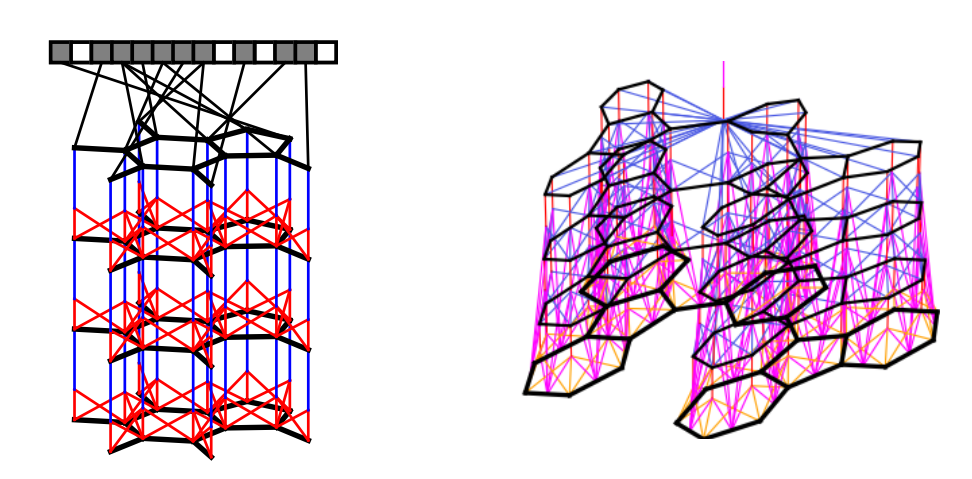
\includegraphics[width=9.5cm]{representations/images/gc1.png}};}
\visible<3->{\node[anchor=west] (im2) at (4.0,3.5){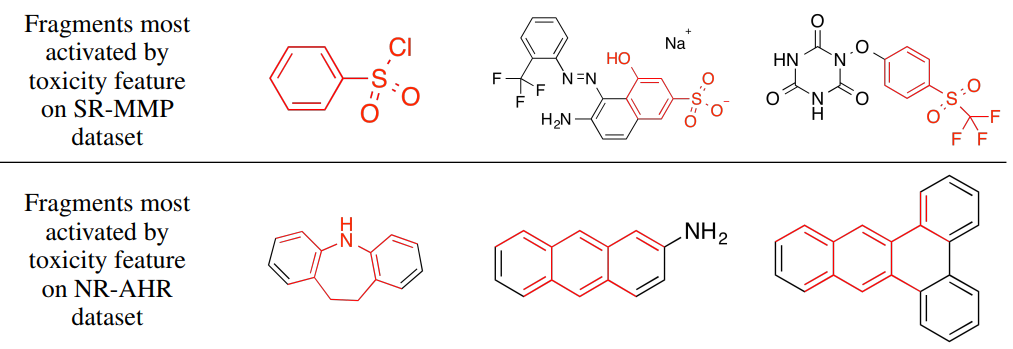
\includegraphics[width=5.5cm]{representations/images/gc2.png}};}
\end{tikzpicture}

\end{center}
